\section{Fractional QHE}

Experiments show, that the filling factor $\nu$ not only takes integer values, but also fractions $\nu=\frac{1}{2}, \frac{2}{5}, ...$.
This can partially be explained with the creation of fractionally charged quasiparticles.
This effect is typically observed for very high magnetic fields.
Since none of the curves goes beyond $\nu = 1$, 
a larger magnetic field would be required to observe fractional filling factors smaller than 1.
In principle, also fractional filling factors larger that one can occur.
Fig. \ref{fig:FQHE} shows the Hall resistivity for $1.4K$ and a gate voltage of $-0.25V$.
There are no plateaus visible at levels of a fractional $\nu$.
The resistivities, where a plateau for $\nu = 4/3$ and $\nu = 5/3$ should be visible, are highlighted as an examlpe.
\begin{figure}[h]
    \centering
    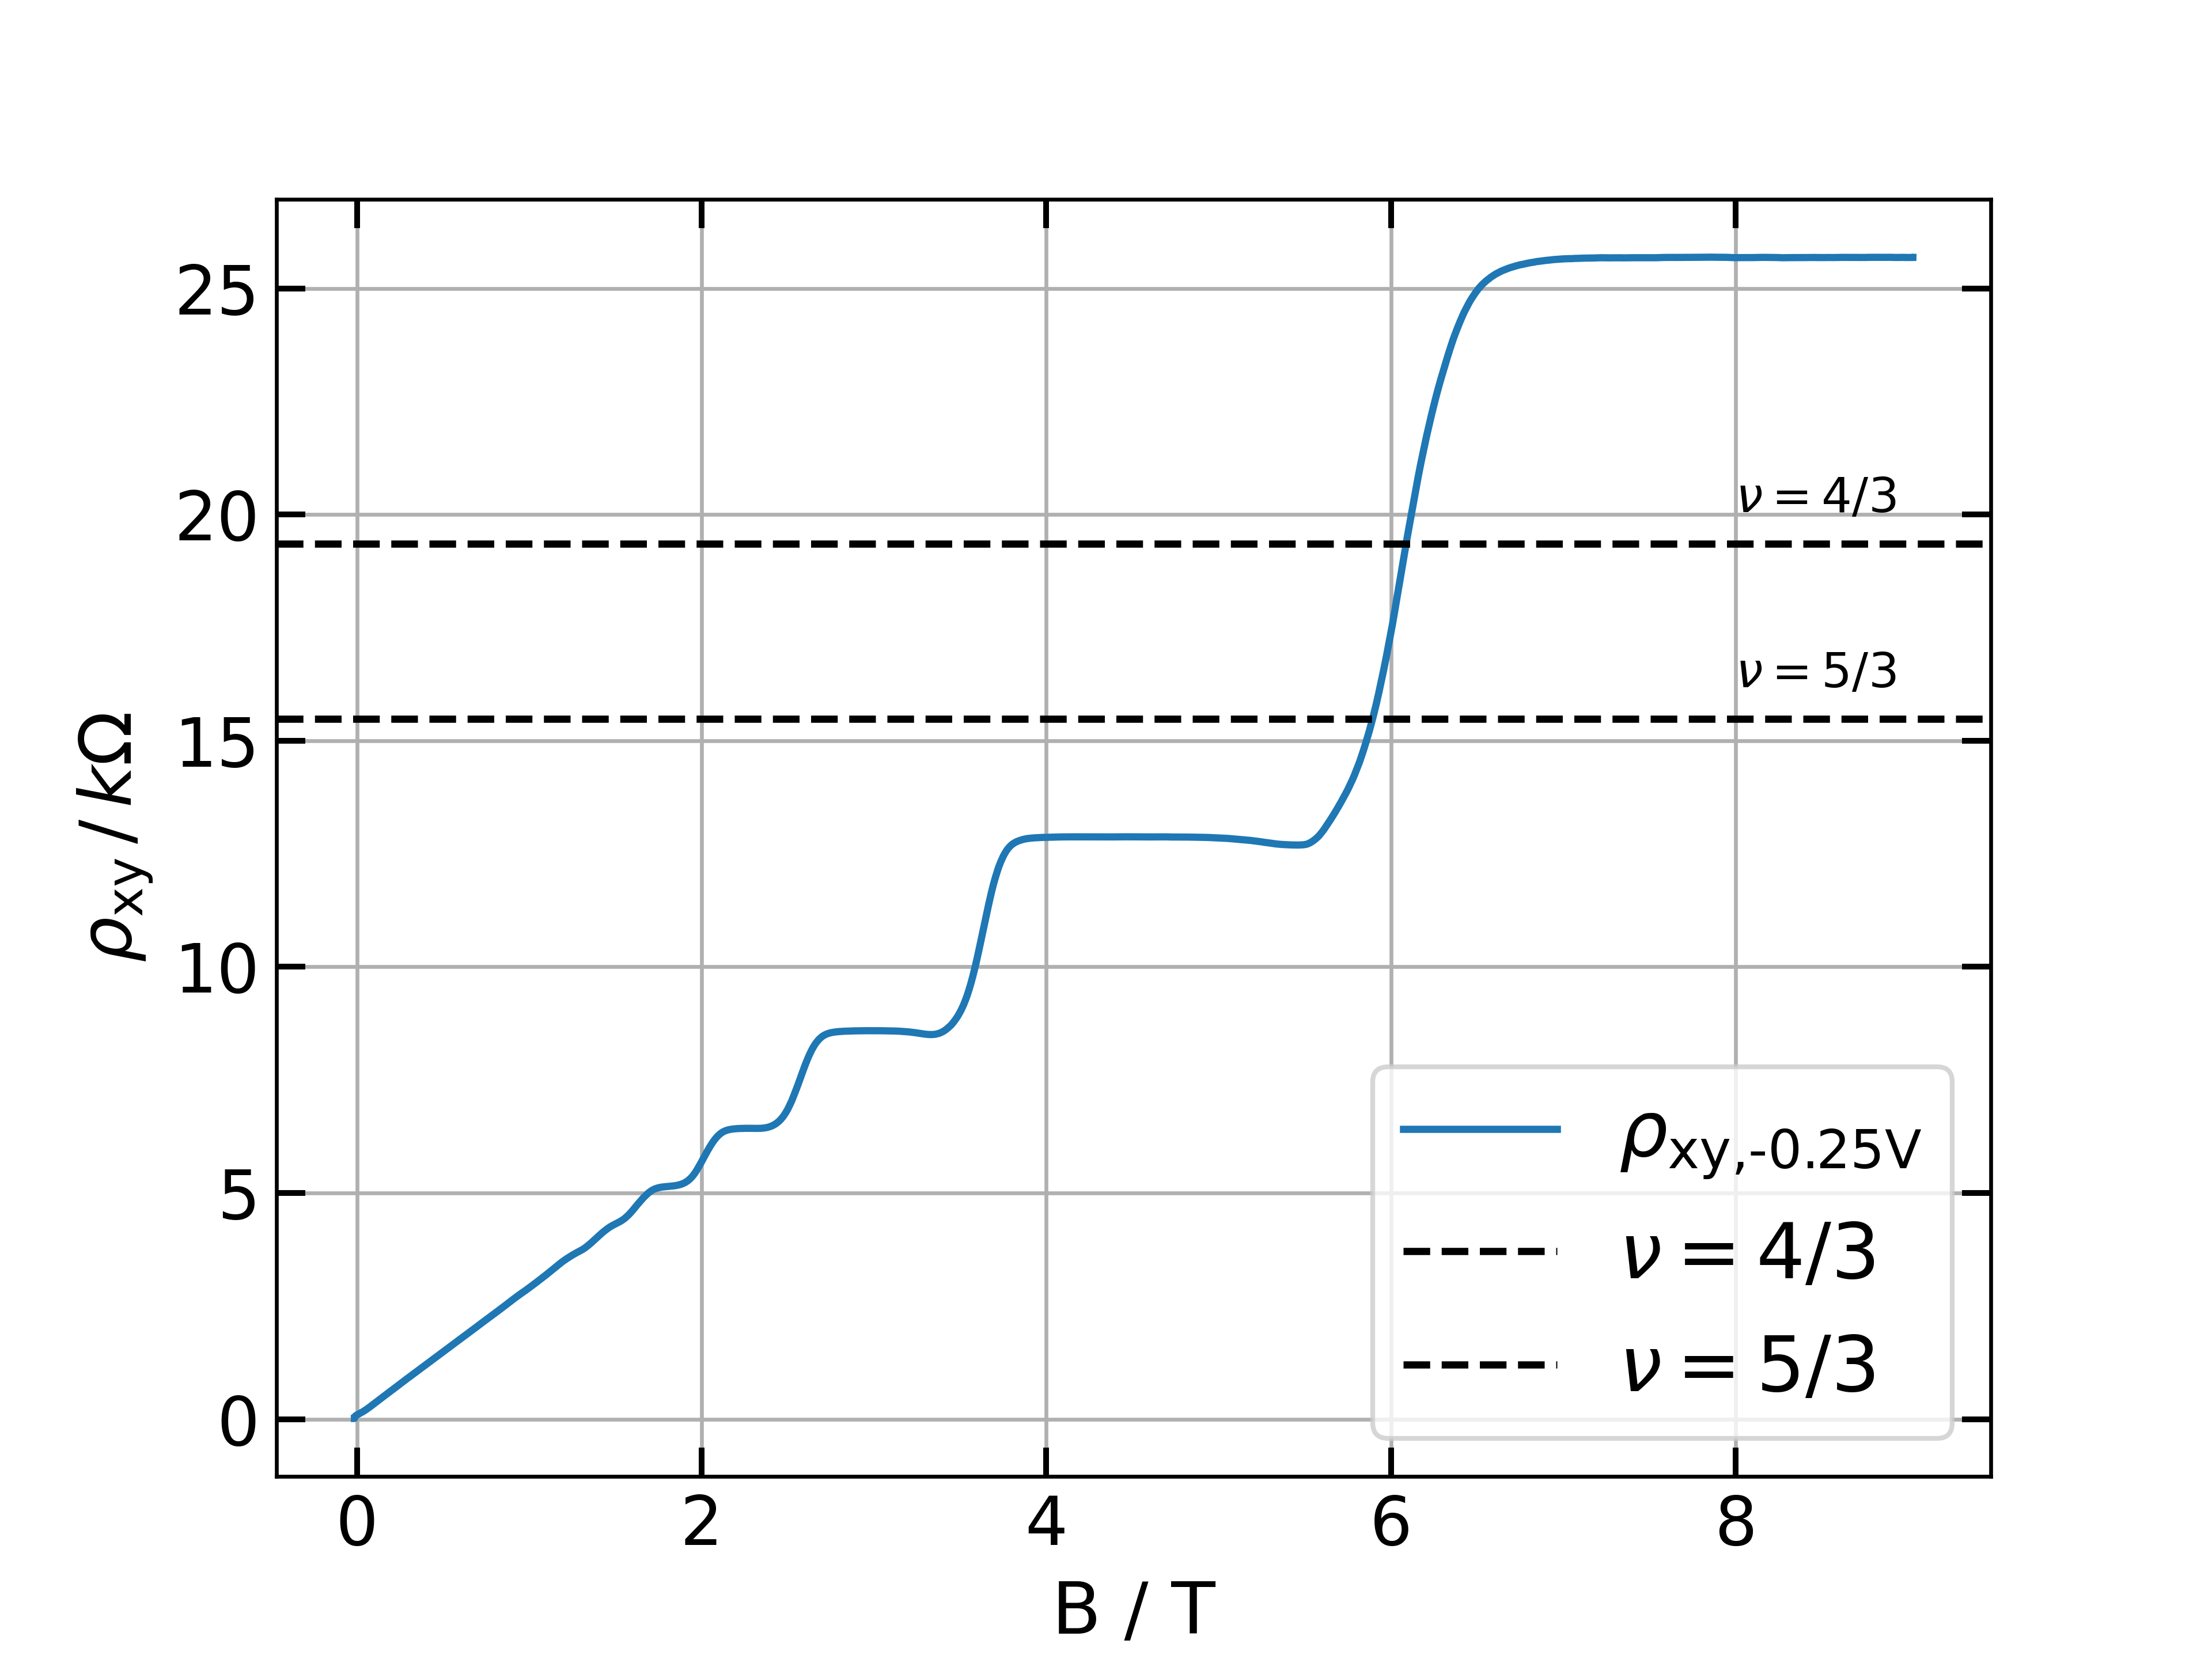
\includegraphics[width=0.45\textwidth]{../Images/FQHE.png}
    \caption{
        }
    \label{fig:FQHE}
\end{figure}
Also the longitudinal resistivity shows no peaks in between the large peaks which correspond to integer valued $\nu$.
To summarise: there are no clear signs of the fractional quantum Hall effect.







